% !TEX program = pdflatex
% Good research programming with AI agents — UMD guest lecture, Aug 31 2026
% Template: TwA Bootcamp (from teaching-ai/slides/ferpa_compliance_segment.tex)
% Timing: 75-min core; optional ~30-min hands-on extension at the end.
\documentclass[aspectratio=169, 10pt]{beamer}

%% ============================================================
%% PACKAGES
%% ============================================================
\usepackage[T1]{fontenc}
\usepackage{lmodern}
\usepackage{graphicx}
\usepackage{booktabs}
\usepackage{array}
\usepackage{tabularx}
\usepackage{colortbl}
\usepackage{tikz}
\usetikzlibrary{positioning, calc, arrows.meta, shapes.geometric, fit, shadows, decorations.pathmorphing}
\usepackage[most]{tcolorbox}
\usepackage{fontawesome5}
\usepackage{hyperref}
\usepackage{multicol}
\usepackage{xcolor}
\usepackage{textcomp}
\usepackage{pifont}

%% ============================================================
%% COLOR DEFINITIONS (TwA Bootcamp palette)
%% ============================================================
\definecolor{UVMGreen}{HTML}{154734}
\definecolor{UVMGold}{HTML}{D4A84B}
\definecolor{SlateTeal}{HTML}{1B4D5C}
\definecolor{DeepCharcoal}{HTML}{2C3E50}
\definecolor{SoftCoral}{HTML}{C0534D}
\definecolor{CoolGray}{HTML}{8899A6}
\definecolor{PaleSage}{HTML}{EDF2F0}
\definecolor{LightGold}{HTML}{FDF6E3}
\definecolor{DarkSlate}{HTML}{0F2B36}

%% ============================================================
%% BEAMER THEME SETUP (TwA template, unchanged)
%% ============================================================
\setbeamercolor{structure}{fg=SlateTeal}
\setbeamercolor{normal text}{fg=DeepCharcoal}
\setbeamercolor{frametitle}{fg=SlateTeal}
\setbeamercolor{title}{fg=SlateTeal}
\setbeamercolor{subtitle}{fg=UVMGold}
\setbeamercolor{author}{fg=DeepCharcoal}
\setbeamercolor{date}{fg=CoolGray}
\setbeamercolor{institute}{fg=CoolGray}
\setbeamercolor{footline}{fg=CoolGray}
\setbeamercolor{block title}{fg=white, bg=SlateTeal}
\setbeamercolor{block body}{bg=PaleSage}
\setbeamercolor{alerted text}{fg=SoftCoral}
\setbeamercolor{item}{fg=SlateTeal}
\setbeamercolor{subitem}{fg=CoolGray}

\setbeamerfont{title}{size=\Large, series=\bfseries}
\setbeamerfont{subtitle}{size=\normalsize}
\setbeamerfont{frametitle}{size=\large, series=\bfseries}
\setbeamerfont{footline}{size=\tiny}

\setbeamertemplate{navigation symbols}{}

\setbeamertemplate{frametitle}{%
  \vskip14pt%
  \nointerlineskip%
  {\usebeamerfont{frametitle}\usebeamercolor[fg]{frametitle}\insertframetitle\par}%
  \vskip2pt%
  {\color{UVMGold}\rule{\textwidth}{1.2pt}}%
  \vskip3pt%
}

\setbeamertemplate{footline}{%
  \begin{beamercolorbox}[wd=\paperwidth, ht=16pt, right, rightskip=1.5cm]{footline}%
    \usebeamerfont{footline}\insertframenumber\,/\,\inserttotalframenumber\vskip3pt%
  \end{beamercolorbox}%
}

\setbeamertemplate{itemize item}{\color{SlateTeal}\raisebox{0.15ex}{\small$\blacktriangleright$}}
\setbeamertemplate{itemize subitem}{\color{CoolGray}\raisebox{0.1ex}{\footnotesize$\bullet$}}

\tcbset{
  keybox/.style={
    colback=PaleSage, colframe=SlateTeal, boxrule=0.8pt, arc=3pt,
    left=6pt, right=6pt, top=4pt, bottom=4pt,
    fonttitle=\bfseries\small\color{white}, coltitle=white, colbacktitle=SlateTeal,
  },
  accentbox/.style={
    colback=LightGold, colframe=UVMGold, boxrule=0.8pt, arc=3pt,
    left=6pt, right=6pt, top=4pt, bottom=4pt,
  },
  quotebox/.style={
    colback=PaleSage, colframe=SlateTeal!50, boxrule=0.5pt, arc=2pt,
    left=8pt, right=8pt, top=4pt, bottom=4pt,
    borderline west={3pt}{0pt}{UVMGold},
  },
  codebox/.style={
    colback=DarkSlate, colframe=DarkSlate, arc=3pt,
    left=8pt, right=8pt, top=6pt, bottom=6pt,
  },
}

% Pop-out aside: a hand-drawn conversation box in the bottom-right corner,
% for the parenthetical remarks that don't belong in the body.
% Wobbly border = two mismatched random-steps strokes (seeded, so it
% compiles identically every time). Usage: \aside{text} or \aside[5cm]{text}
% Text uses the Augie handwriting font when installed (tlmgr install augie);
% falls back to italic otherwise.
\IfFileExists{t1augie.fd}%
  {\newcommand{\asidefont}{\normalsize\fontfamily{augie}\selectfont\hyphenpenalty=10000\exhyphenpenalty=10000}}%
  {\newcommand{\asidefont}{\footnotesize\itshape\hyphenpenalty=10000\exhyphenpenalty=10000}}
\newcommand{\aside}[2][4.2cm]{%
\begin{tikzpicture}[remember picture, overlay]
  \pgfmathsetseed{4242}%
  \node[anchor=south east, xshift=-1.5cm, yshift=0.6cm,
        fill=LightGold, rounded corners=9pt,
        text=DeepCharcoal, font=\asidefont, align=left,
        text width=#1, inner sep=9pt]
    (asidebox) at (current page.south east) {#2};
  \draw[DeepCharcoal, line width=1.0pt, rounded corners=11pt,
        decorate, decoration={random steps, segment length=10pt, amplitude=1.2pt}]
    ($(asidebox.south west)+(-2pt,-2pt)$) rectangle ($(asidebox.north east)+(2pt,2pt)$);
  \draw[DeepCharcoal!70, line width=0.6pt, rounded corners=10pt,
        decorate, decoration={random steps, segment length=14pt, amplitude=1.8pt}]
    ($(asidebox.south west)+(-3pt,-1pt)$) rectangle ($(asidebox.north east)+(1pt,3pt)$);
\end{tikzpicture}}

% Section divider helper
\newcommand{\divider}[2]{%
{\setbeamertemplate{footline}{}%
\begin{frame}[plain]
\begin{tikzpicture}[remember picture, overlay]
  \fill[SlateTeal] (current page.north west) rectangle (current page.south east);
  \fill[UVMGold] ([yshift=0.3cm]current page.center -| current page.west) rectangle ([yshift=0.25cm]current page.center -| current page.east);
  \node[anchor=center, text=white, font=\fontsize{24}{30}\bfseries\selectfont]
    at ([yshift=1.6cm]current page.center) {#1};
  \node[anchor=center, text=UVMGold, font=\fontsize{12}{16}\selectfont]
    at ([yshift=-0.8cm]current page.center) {#2};
\end{tikzpicture}
\end{frame}}%
}

\title{Good research programming with AI agents}
\author{Emily Beam}
\institute{Department of Economics, University of Vermont}
\date{August 31, 2026}

\begin{document}

%% ====== TITLE ======
{
\setbeamertemplate{footline}{}
\begin{frame}[plain]
\begin{tikzpicture}[remember picture, overlay]
  \fill[SlateTeal] (current page.north west) rectangle (current page.south east);
  \fill[UVMGold] ([yshift=0.3cm]current page.center -| current page.west) rectangle ([yshift=0.25cm]current page.center -| current page.east);
  \node[anchor=center, text=white, font=\fontsize{25}{31}\bfseries\selectfont, align=center]
    at ([yshift=2.2cm]current page.center) {Good research programming\\with AI agents};
  \node[anchor=center, text=UVMGold, font=\fontsize{13}{17}\selectfont]
    at ([yshift=0.9cm]current page.center) {Building your LSMS project so it lasts};
  \node[anchor=center, text=white!80, font=\fontsize{10}{12}\selectfont]
    at ([yshift=-1.3cm]current page.center) {Emily Beam $\cdot$ University of Vermont};
  \node[anchor=center, text=CoolGray, font=\fontsize{9}{11}\selectfont]
    at ([yshift=-2.0cm]current page.center) {UMD Development Economics $\cdot$ August 31, 2026};
\end{tikzpicture}
\end{frame}
}

%% ====== TODAY'S PLAN ======
\begin{frame}{Today's plan}

\begin{enumerate}
  \item Why programming is a research skill
  \item Setting up your project
  \item Git in fifteen minutes
  \item Working with an AI agent
  \item Live demo
  \item Rules of the road --- and setup triage
\end{enumerate}

\vspace{0.4cm}

\begin{tcolorbox}[accentbox]
\centering
Everything from today lives at \textbf{\url{github.com/eabeam/umd-dev-econ-ai}} --- slides, templates, cheat sheets, and the setup guide.
\end{tcolorbox}

\end{frame}

%% ====== 1. WHY ======
\divider{Why programming is a research skill}{(and not just a chore before the economics starts)}

\begin{frame}{Your semester project is a small research paper}

\begin{center}
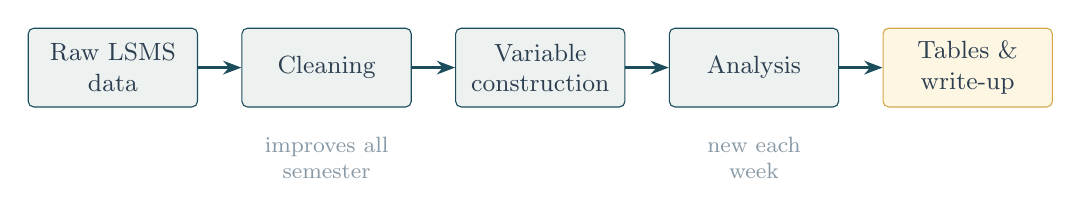
\begin{tikzpicture}[
  box/.style={rectangle, rounded corners=2pt, draw=SlateTeal, fill=PaleSage, text=DeepCharcoal,
              minimum height=1.0cm, minimum width=2.15cm, align=center, font=\small},
  resultbox/.style={rectangle, rounded corners=2pt, draw=UVMGold, fill=LightGold, text=DeepCharcoal,
              minimum height=1.0cm, minimum width=2.15cm, align=center, font=\small},
  arrow/.style={-{Stealth}, thick, SlateTeal},
  node distance=0.55cm
]
  \node[box] (raw) {Raw LSMS\\data};
  \node[box, right=of raw] (clean) {Cleaning};
  \node[box, right=of clean] (construct) {Variable\\construction};
  \node[box, right=of construct] (analysis) {Analysis};
  \node[resultbox, right=of analysis] (table) {Tables \&\\write-up};
  \draw[arrow] (raw) -- (clean);
  \draw[arrow] (clean) -- (construct);
  \draw[arrow] (construct) -- (analysis);
  \draw[arrow] (analysis) -- (table);
  \node[below=0.25cm of clean, text=CoolGray, font=\footnotesize, align=center] {improves all\\semester};
  \node[below=0.25cm of analysis, text=CoolGray, font=\footnotesize, align=center] {new each\\week};
\end{tikzpicture}
\end{center}

\vspace{0.3cm}

\begin{itemize}
  \item Twelve assignments, one survey, one growing pipeline --- the same shape as a real paper
  \item Your cleaning code is an \textbf{investment}: it compounds from Assignment 1 to Assignment 12
  \item By December, this could be the empirical base of your second-year paper
\end{itemize}

\end{frame}

\begin{frame}{The product isn't the table --- it's the pipeline that makes it}

From your assignment:

\begin{tcolorbox}[quotebox]
\textit{``...files that could reproduce every table/figure from your submissions without editing the code other than setting the project directory.''}
\end{tcolorbox}

\vspace{0.3cm}

That single sentence is a complete replicability standard. It means:

\begin{itemize}
  \item Someone else (including you, later) can \textbf{rerun everything} from raw data to final table
  \item No ``oh, you also have to run this other file first'' --- the code \textbf{documents itself}
  \item If a number in your write-up can't be reproduced, it isn't a result yet
\end{itemize}

\end{frame}

\begin{frame}{What changes with AI: verifying becomes the bottleneck}

\begin{itemize}
  \item With an agent, you will produce working code \textbf{faster than you can understand it}
  \item The constraint moves: not \emph{can I write this loop?} but \emph{is this pipeline doing what I think?}
  \item Good structure, version control, and documentation are how you keep up
\end{itemize}

\vspace{0.4cm}

\begin{tcolorbox}[accentbox]
\centering
Everything in this lecture is a \textbf{verification} tool. The AI writes more; you check better.
\end{tcolorbox}

\end{frame}

%% ====== 2. PROJECT SETUP ======
\divider{Setting up your project}{one folder, clear paths, files that explain themselves}

\begin{frame}[fragile]{One folder, one project}

\begin{columns}[T]
\begin{column}{0.42\textwidth}
\begin{tcolorbox}[codebox]
\color{white}\footnotesize\ttfamily
lsms-project/\\
\hspace*{1em}config.do\\
\hspace*{1em}code/\\
\hspace*{2em}cleaning/\\
\hspace*{2em}analysis/\\
\hspace*{1em}data/\hspace*{1em}{\color{CoolGray}(never in Git)}\\
\hspace*{2em}raw/\\
\hspace*{2em}clean/\\
\hspace*{1em}output/\\
\hspace*{1em}README.md
\end{tcolorbox}
\end{column}
\begin{column}{0.54\textwidth}
\begin{itemize}
  \item \textbf{raw/} is read-only --- you never edit a file the World Bank gave you
  \item \textbf{cleaning/} writes to data/clean/; \textbf{analysis/} reads from it
  \item \textbf{data/} stays out of Git --- the \texttt{.gitignore} template in the class repo handles this
  \item The agent sees this structure too --- a tidy folder is a better prompt than any instruction
\end{itemize}
\end{column}
\end{columns}

\end{frame}

\begin{frame}[fragile]{Hardcode nothing: the config pattern}

The only line a replicator should ever edit:

\begin{tcolorbox}[codebox]
\color{white}\footnotesize\ttfamily
* config.do --- the ONE file with a path in it\\
global root "C:/Users/you/Documents/lsms-project"\\[6pt]
* every other file starts with:\\
include config.do\\
use "\$root/data/clean/household.dta", clear
\end{tcolorbox}

\vspace{0.3cm}

\begin{itemize}
  \item A path like \texttt{C:/Users/you/Desktop/final/actually\_final/} breaks on every machine but yours
  \item This is exactly the ``setting the project directory'' your assignment allows --- one edit, everything runs
\end{itemize}

\end{frame}

\begin{frame}{Cleaning files build; analysis files stand alone}

\begin{columns}[T]
\begin{column}{0.48\textwidth}
\begin{tcolorbox}[keybox, title={\faLayerGroup\quad Cleaning files}]
\footnotesize
Build datasets, get reused, get \textbf{better} all semester\\[4pt]
Improving a variable definition in week 6? Fine --- that's the design. Rerun, and every table updates.
\end{tcolorbox}
\end{column}
\begin{column}{0.48\textwidth}
\begin{tcolorbox}[keybox, title={\faFile\quad Analysis files}]
\footnotesize
One file per table or figure, \textbf{self-contained}\\[4pt]
It may call cleaning output --- but running it alone produces the table. (Your grader thanks you. So does your November self.)
\end{tcolorbox}
\end{column}
\end{columns}

\vspace{0.35cm}

\begin{tcolorbox}[accentbox]
\centering
This split is in your assignment already --- it's also how most co-authored research code is organized.
\end{tcolorbox}

\end{frame}

\begin{frame}[fragile]{Readable code (your coauthor is you, in November)}

\begin{columns}[T]
\begin{column}{0.48\textwidth}
\begin{tcolorbox}[codebox]
\color{SoftCoral}\footnotesize\ttfamily
gen x2 = x1*sh\_m/tot if f==1\\
replace x2 = 0 if x2==.
\end{tcolorbox}
\end{column}
\begin{column}{0.48\textwidth}
\begin{tcolorbox}[codebox]
\color{white}\footnotesize\ttfamily
* Per-capita food exp., members\\
* present >6 mo (BID def., p.12)\\
gen foodexp\_pc = foodexp\_hh /\\
\hspace*{2em}n\_members\_present
\end{tcolorbox}
\end{column}
\end{columns}

\vspace{0.35cm}

\begin{itemize}
  \item Names carry meaning; comments say \textbf{why}, not what
  \item The test: open a file cold --- can you tell what it does in thirty seconds?
  \item Agents inherit your standards --- messy in, messy out
\end{itemize}

\aside[6.2cm]{November-you has no memory of August-you. None.}

\end{frame}

%% ====== 3. GIT ======
\divider{Git in fifteen minutes}{a lab notebook for your code}

\begin{frame}{Git: Dropbox with perfect version control}

You already use the pieces --- Git puts them together, for code:

\vspace{0.15cm}

\begin{columns}[T]
\begin{column}{0.31\textwidth}
\begin{tcolorbox}[keybox, title={\faCloud\quad Like Dropbox}]
\footnotesize
Your project, backed up and synced\\[4pt]
But a version saves \textbf{when you say so}, with a label --- and no version ever overwrites another. (No more \texttt{final\_v2\_REAL.do}.)
\end{tcolorbox}
\end{column}
\begin{column}{0.31\textwidth}
\begin{tcolorbox}[keybox, title={\faEdit\quad Like track changes}]
\footnotesize
Every edit shows up as a \textbf{diff}: what changed, who changed it, and --- if the message is good --- why\\[4pt]
Accept or reject, same as in Word
\end{tcolorbox}
\end{column}
\begin{column}{0.31\textwidth}
\begin{tcolorbox}[keybox, title={\faCodeBranch\quad Plus branches}]
\footnotesize
The genuinely new trick: a \textbf{parallel copy} of the whole project\\[4pt]
Try the risky idea there; merge it back if it works (delete it quietly if it doesn't)
\end{tcolorbox}
\end{column}
\end{columns}

\vspace{0.3cm}

\begin{tcolorbox}[accentbox]
\small This is also how you stay \textbf{in control of an agent}: in a plain folder, its edits just happen --- in Git, they arrive as diffs \textbf{you} review. And it's how every co-authored code base survives. Worth the skill.
\end{tcolorbox}

\end{frame}

\begin{frame}[fragile]{The whole loop is four commands}

\begin{tcolorbox}[codebox]
\color{white}\small\ttfamily
git add .\hspace{2.6em}{\color{CoolGray}stage what changed}\\
git commit\hspace{1.9em}{\color{CoolGray}snapshot it, with a message}\\
git push\hspace{3.2em}{\color{CoolGray}back it up to GitHub}\\
git log\hspace{3.9em}{\color{CoolGray}see the story so far}
\end{tcolorbox}

\vspace{0.3cm}

\begin{itemize}
  \item In VS Code, this is the \textbf{Source Control panel} --- type a message, click commit, click sync
  \item Commit \textbf{when a thing works}: after each table, after each cleaning step (not once a month)
  \item Message guide and cheat sheet are in the class repo --- keep the cheat sheet open for a few weeks
\end{itemize}

\end{frame}

\begin{frame}{Your undo button: Git while the agent works}

\begin{itemize}
  \item Every file the agent touches shows up marked in the \textbf{Source Control panel} --- click it for a side-by-side diff of exactly what changed
  \item \textbf{Commit before} handing the agent a big task --- a clean checkpoint turns \emph{Discard All Changes} into a real undo button
  \item Agent went sideways? Discard, sharpen the prompt, run it again
  \item \textbf{Commit after} each thing that works --- small commits keep agent work reviewable
\end{itemize}

\vspace{0.3cm}

\begin{tcolorbox}[accentbox, width=0.66\textwidth]
The rhythm: \textbf{checkpoint $\to$ delegate $\to$ read the diff $\to$ keep or discard.} You are never stuck with what the agent did.
\end{tcolorbox}

\aside[3.6cm]{Discarding isn't defeat --- it's cheaper than repair.}

\end{frame}

\begin{frame}[fragile]{Reading a diff is a research skill}

What Git shows you when a file changes:

\begin{tcolorbox}[codebox]
\footnotesize\ttfamily
\color{SoftCoral}- drop if age < 15\\
\color{white}+ drop if age < 18\\[4pt]
\color{SoftCoral}- gen employed = (hours > 0)\\
\color{white}+ gen employed = (hours > 0) \& !missing(hours)
\end{tcolorbox}

\vspace{0.3cm}

\begin{itemize}
  \item Two changed lines --- and your sample and your employment rate both just moved
  \item \textbf{This is how you audit an agent}: it edits, you read the diff before accepting
  \item If a diff changes your N and the commit message doesn't say why, that's a finding
\end{itemize}

\end{frame}

\begin{frame}{Encouraged, not graded}

\begin{itemize}
  \item The deal from your syllabus: Git is \textbf{encouraged}, and skipping it costs you nothing on grades
  \item My pitch anyway: this is the lowest-effort week to start --- empty project, nothing to lose, whole semester to benefit
  \item Your repo also travels with you --- to Econ 616, your summer paper, your job market code sample
\end{itemize}

\vspace{0.4cm}

\begin{tcolorbox}[accentbox]
\centering
In the repo: \textbf{git cheat sheet} $\cdot$ \textbf{commit message guide} $\cdot$ \textbf{.gitignore} template for econ projects
\end{tcolorbox}

\end{frame}

%% ====== 4. AI AGENT ======
\divider{Working with an AI agent}{three rungs of delegation --- and what each one asks of you}

\begin{frame}{Three rungs of delegation (all inside VS Code)}

\begin{columns}[T]
\begin{column}{0.31\textwidth}
\begin{tcolorbox}[keybox, title={1 $\cdot$ Completions}]
\footnotesize
Ghost text finishes your line as you type (Copilot)\\[4pt]
\textbf{Good for}: boilerplate, finishing table code you started
\end{tcolorbox}
\end{column}
\begin{column}{0.31\textwidth}
\begin{tcolorbox}[keybox, title={2 $\cdot$ Scoped edits}]
\footnotesize
Highlight code, ask the panel: explain this, fix this\\[4pt]
\textbf{Good for}: debugging, understanding documentation
\end{tcolorbox}
\end{column}
\begin{column}{0.31\textwidth}
\begin{tcolorbox}[keybox, title={3 $\cdot$ Agent mode}]
\footnotesize
``Build a weighted summary table from this module'' (Codex)\\[4pt]
\textbf{Good for}: multi-file work, scaffolding, first drafts of pipelines
\end{tcolorbox}
\end{column}
\end{columns}

\vspace{0.35cm}

\begin{itemize}
  \item One window: the panel, the ghost text, and the terminal all live in VS Code
  \item Different tools sit on different rungs --- Copilot low, Codex high --- but the rungs are what matter
\end{itemize}

\end{frame}

\begin{frame}{While you're in VS Code anyway}

Not AI --- just things the same window does well:

\vspace{0.15cm}

\begin{itemize}
  \item \textbf{LaTeX} --- the LaTeX Workshop extension compiles your paper right next to your code (and yes, the agent can edit \texttt{.tex} too)
  \item \textbf{Markdown preview} --- your README and decisions log, rendered as you type
  \item \textbf{Stata syntax highlighting} --- search the extensions marketplace for ``Stata''
  \item \textbf{Project-wide search} --- every file, one keystroke (where did I define \texttt{foodexp\_pc}?)
\end{itemize}

\vspace{0.3cm}

\begin{tcolorbox}[accentbox]
\centering
The point isn't any one feature --- it's that your \textbf{whole project} lives in one place the agent can also see.
\end{tcolorbox}

\end{frame}

\begin{frame}[fragile]{The higher the rung, the heavier your verification}

\begin{itemize}
  \item A completion you watched appear needs a glance; an agent-built pipeline needs an \textbf{audit}
  \item The agent can even run Stata itself --- batch mode, then it reads the log and fixes its own errors:
\end{itemize}

\begin{tcolorbox}[codebox]
\color{white}\small\ttfamily
stata-mp -b do build\_table1.do\hspace{2em}{\color{CoolGray}writes build\_table1.log}
\end{tcolorbox}

\vspace{0.3cm}

\begin{itemize}
  \item Which is genuinely useful! And means code can now go from ``asked'' to ``done'' \textbf{without passing through your head}
  \item The two things that go wrong next have nothing to do with syntax errors...
\end{itemize}

\end{frame}

\begin{frame}{Failure mode 1: it runs, but nobody can read it}

\begin{itemize}
  \item Agent code is rarely \emph{wrong} --- it's \textbf{unreadable}: fifteen clever lines where four plain ones would do
  \item Unreadable code can't be checked by a coauthor, a referee, or you-in-November
  \item The fix is cheap: tell the agent your standards --- ``plain Stata, comment the why, match the style of \texttt{clean\_household.do}''
\end{itemize}

\vspace{0.4cm}

\begin{tcolorbox}[accentbox]
\centering
Agents follow the house style you give them. No house style, no house.
\end{tcolorbox}

\end{frame}

\begin{frame}{Failure mode 2: silent research decisions}

A true story, lightly anonymized:

\begin{tcolorbox}[quotebox]
An agent, asked to build an analysis dataset, quietly \textbf{imputed missing values at the mean} --- so no observations dropped, N never jumped around, and the usual tell that something happened to the sample... never happened.
\end{tcolorbox}

\vspace{0.3cm}

\begin{itemize}
  \item Imputing, dropping, winsorizing, recoding --- these are \textbf{research decisions}, not programming details
  \item An agent will make them for you, competently and silently
  \item The habit: a \textbf{decisions log} with every assignment --- what you found, what you did, what it cost. (Template in the repo; it's one table.)
\end{itemize}

\vspace{0.2cm}

\begin{center}
\small\color{CoolGray}\textit{Every cleaning decision is a research decision. If you can't justify it, don't ship it.}
\end{center}

\end{frame}

%% ====== 5. DEMO ======
\divider{Live demo}{Assignment 1, the real way}

\begin{frame}{What you're about to see}

\begin{enumerate}
  \item Open the project folder in VS Code --- agent reads the survey documentation with me
  \item Agent mode: build a weighted household summary table from one LSMS module
  \item The agent runs Stata itself (batch mode), reads the log, fixes its own error
  \item We read the \textbf{diff} before accepting anything
  \item We catch it making a silent decision --- and log it
  \item Commit. The whole loop, start to finish.
\end{enumerate}

\vspace{0.3cm}

\begin{tcolorbox}[accentbox]
\centering
Watch for step 5. It will try something reasonable-looking. That's the point.
\end{tcolorbox}

\end{frame}

\begin{frame}{The other way (sixty seconds)}

For contrast: the same task, by pasting code into a chat window in the browser.

\vspace{0.2cm}

\begin{itemize}
  \item No files --- it can't see your data, your documentation, or your other code
  \item No diffs --- changes arrive as a wall of text you paste over your work
  \item No history --- next week, you cannot reconstruct what you did
\end{itemize}

\vspace{0.3cm}

\begin{tcolorbox}[accentbox]
\centering
It works --- until the first time you need to know \textbf{what you did}. In research, that time always comes.
\end{tcolorbox}

\end{frame}

%% ====== 6. RULES ======
\divider{Rules of the road}{and what to do this week}

\begin{frame}{The AI policy, in one slide}

\begin{columns}[T]
\begin{column}{0.48\textwidth}
\begin{tcolorbox}[keybox, title={\faCheckCircle\quad Yes}]
\footnotesize
Programming assistance $\cdot$ debugging $\cdot$ explaining documentation $\cdot$ brainstorming approaches $\cdot$ proofreading your write-ups
\end{tcolorbox}
\end{column}
\begin{column}{0.48\textwidth}
\begin{tcolorbox}[keybox, title={\faTimesCircle\quad No}]
\footnotesize
Generating the text you submit $\cdot$ interpreting your tables $\cdot$ doing the analytical thinking
\end{tcolorbox}
\end{column}
\end{columns}

\vspace{0.35cm}

\begin{tcolorbox}[accentbox]
\centering
And always: \textbf{verify every result, understand every line.} The tables are yours to explain in class --- that's the real enforcement mechanism.
\end{tcolorbox}

\end{frame}

\begin{frame}{This week}

\begin{enumerate}
  \item \textbf{World Bank microdata account} --- today, if you haven't. Approval takes days, and Assignment 1 needs it.
  \item Finish the \textbf{setup guide} (repo): ChatGPT plan, VS Code + Codex, Git, GitHub, your project repo
  \item Run the \textbf{five-minute test} at the end of the guide --- if all four steps work, you're ready
  \item Stuck? Note where, and bring it to class --- setup triage is part of the plan, not a failure
\end{enumerate}

\vspace{0.35cm}

\begin{tcolorbox}[accentbox]
\centering
\textbf{github.com/eabeam/umd-dev-econ-ai} --- setup guide, templates, cheat sheets, these slides.\\[3pt]
The loop to remember: \textbf{agent writes $\to$ you review $\to$ it runs $\to$ you check $\to$ you commit}.
\end{tcolorbox}

\end{frame}

%% ====== OPTIONAL EXTENSION ======
\divider{If we have time: you drive}{one prompt, one commit, before you leave}

\begin{frame}{Your turn}

Each of you, on your own machine, with the demo data:

\vspace{0.2cm}

\begin{enumerate}
  \item Open your project folder in VS Code
  \item Give the agent one prompt (I'll give you a menu --- all Assignment-1-shaped)
  \item Read the diff. Actually read it!
  \item Run the result, check the output, commit
\end{enumerate}

\vspace{0.3cm}

\begin{itemize}
  \item If it works: your setup is verified before Assignment 1 is even due
  \item If it doesn't: even better --- we fix it now, together, instead of Sunday night
\end{itemize}

\end{frame}

\end{document}
